\documentclass{bmstu}
\lstset{%
	language=cxx,   					% выбор языка для подсветки	
	basicstyle=\small\sffamily,			% размер и начертание шрифта для подсветки кода
	numbers=left,						% где поставить нумерацию строк (слева\справа)
	%numberstyle=,						% размер шрифта для номеров строк
	stepnumber=1,						% размер шага между двумя номерами строк
	numbersep=5pt,						% как далеко отстоят номера строк от подсвечиваемого кода
	frame=single,						% рисовать рамку вокруг кода
	tabsize=4,							% размер табуляции по умолчанию равен 4 пробелам
	captionpos=t,						% позиция заголовка вверху [t] или внизу [b]
	breaklines=true,					
	breakatwhitespace=true,				% переносить строки только если есть пробел
	escapeinside={\#*}{*)},				% если нужно добавить комментарии в коде
	backgroundcolor=\color{white},
}

\usepackage{pdfpages}

\bibliography{biblio}

\renewcommand{\labelitemi}{\labelitemfont---}
\renewcommand{\labelitemii}{\labelitemfont---}
\renewcommand{\labelitemiii}{\labelitemfont---}

\makeatletter
\renewcommand{\l@section}{\@dottedtocline{1}{0em}{1.8em}}
\renewcommand{\l@subsection}{\@dottedtocline{2}{0em}{2.3em}}
\makeatother



\usepackage{amssymb}

\begin{document}

\makecourseworktitle
{Информатика и системы управления}
{Программное обеспечение ЭВМ и информационные технологии}
{Моделирование сцены улицы из библиотеки объектов}
{Козырнов~А.~Д./ИУ7-52Б}
{Мартынюк~Н.~Н.}
{}


\maketableofcontents


%\begin{definitions}
	\definition{}{}
\end{definitions}
%\begin{abbreviations}
	\definition{}{}
\end{abbreviations}

\chapter*{ВВЕДЕНИЕ}
\addcontentsline{toc}{chapter}{ВВЕДЕНИЕ}


В настоящее время компьютерное графическое моделирование
используется для уменьшений недопониманий между заказчиком и исполнителем.
С его помощью можно заранее определить детали проекта.

\textbf{Цель курсовой работы} --- моделирование сцены улицы из разработанной библиотеки
объектов (дома разной этажности, заправка, светофор) и предоставление возможности изменить
положение камеры и источника света, а также сохранение и просмотр разработанных сцен. Для
решения поставленной цели необходимо выполнить следующие задачи:
\begin{itemize}
    \item выбрать алгоритмы компьютерной графики для визуализации трехмерной
        сцены;
    \item выбрать язык программирования и среду разработки;
    \item разработать программное обеспечение и реализовать выбранные алгоритмы визуализации;
    \item провести замеры временных характеристик разработанного программного обеспечения.
\end{itemize}



\chapter{Аналитический раздел}

В данном разделе проводится выбор и анализ существующих алгоритмов построения изображения
трехмерной сцены.


\section{Описание объектов сцены}

Сцена состоит из набора следующих объектов:
\begin{itemize}
    \item Площадка --- правильный параллелипипед, состоящий из сетки ячеек, на
        которой размещаются объекты сцены. Размеры площадки задаются по ширине и 
        длине одновременно. Ячейка --- заранее определенный объект, определенный внутри
        программы;

    \item Объект сцены --- модель, расположенная на ячейке сцены. Данные объекты
        могут занимать только одну ячейку сцены одновременно. Каждая такая модель
        описана массивом граней с нормалями. Все доступные объекты сцены
        определены заранее, и в программе не предусмотрена возможность изменения
        старых и добавления новых объектов сцены. Данные модели можно
        перемещать по сцене и вращать относительно их заданного центра.

    \item Источник света --- точка в пространстве. Источник света имеет координаты,
        направление и интенсивность освещения. В зависимости от расположения
        и направления источника света относительно камеры определяются тени от объектов
        сцены.

    \item Камера --- точка в пространстве. От ее положения и направления взгляда
        пользователь может наблюдать сцену с определенного ракурса. При изменении
        положения или направления камеры, обзор на сцену изменяется.
\end{itemize}

\section{Анализ способов задания моделей}

В компьютерной графике способов задания моделей три: каркасная, поверхностная и
объемная~\cite{prilipenko:2005}.

%\subsection{Каркасная модель}

Каркасная модель представляется набором вершин и ребер, соединяющих вершины.
Данное представление не всегда точно передает информацию об объектах сцены,
так как может неоднозначно определять его форму.

%\subsection{Поверхностная модель}

Поверхностная модель --- это модель, которая каким-либо образом задана поверхностями.
Описание прверхности может быть аналитическим или с помощью полигонов.

%\subsection{Объемная (твердотельная) модель}

Твердотельная форма задания модели отличается от поверхностной тем, что в таких моделях
задается информация о материале объекта.

\subsection{Выбор способа задания модели}

Для решения поставленной задачи необходимо правильное восприятие форм объекта, поэтому
каркасная модель не подходит для решения поставленной задачи. Твердотельная модель также не
подходит для решения задачи, так как неважно из чего состоят объекты сцены. Поверхностная
модель точно определяет форму объекта сцены, поэтому в данной программе можноиспользовать
поверхностную модель.


\section{Анализ алгоритмов удаления невидимых ребер и граней}

В компьюетрной графике важнейшей задачей является удаление невидимых ребер и граней.
Данные алгоритмы определяют, какие ребра и грани видны наблюдателю, находящегося
в определенной точке пространства относительно этих ребер и граней.

Алгоритмы делятся на способы решения. Первая группа алгоритмов решают задачу
в объектом пространстве, другие --- задачу в пространстве изображения.
Алгоритмы, работающие с объектным пространством,  дают более точные результаты,
однако медленнее алгоритмов, работающих в пространстве изображения.

\subsection{Алгоритм Робертса}

Данный алгоритм работает в объектном пространтсве. Решает задачу только с выпуклыми телами.
Алгоритм выполняется в 4 этапа~\cite{roberts:1964}:
\begin{itemize}
    \item подготовка исходных данных --- разбиение невыпуклых объектов на выпуклые, составление
        матрицы тела каждого из объектов;
    \item удаление ребер, экранируемых самим телом;
    \item удаление ребер, экранируемых другими телами;
    \item удаление линий пересечения тел, экранируемых
        самими телами и другими телами, связанными отношением протыкания.
\end{itemize}



\textbf{Преимущества}:
\begin{itemize}
    \item высокая точность определения видимости граней без приближений.
\end{itemize}


\textbf{Недостатки}:
\begin{itemize}
    \item Тела сцены должны быть выпуклыми, что не всегда так.
    \item Высокая вычислительная сложность при большом количестве граней. Рост
        вычислительной сложности --- квадрат количества граней.
\end{itemize}

\subsection{Z-буфер}

Данный подход работает в пространстве изображения.

Алгоритм Z-буфер~\cite{zbuffer:1974} использует два буфера: буфер глубины и буфер кадра.

Буфер глубины определяет для каждого пикселя информацию о глубине ближайшего к наблюдателю
объекта.  В буфере кадра хранится цвет пикселей.

\medskip

Алгоритм начинает работу с инициализации буфера глубины максимальным значением глубины.
При растеризации (отрисовке) каждого полигона вычисляется глубина каждого из его пикселей.
Если глубина очередного пикселя меньше соответствующей глубины в буфере глубины, то
изменяется соответствующая информация в буфере кадра и значение глубины этого пикселя
обновляется.

\textbf{Преимущества}:
\begin{itemize}
    \item возможность отрисовки объектов любой сложности;
    \item Линейная зависимость от количества пикселей, отрисовываемых на изображении;
    \item простота реализации.
\end{itemize}

\textbf{Недостатки}:
\begin{itemize}
    \item необходима дополнительная память для хранения буфера глубины;
    \item возможны артефакты при недостаточной точности буфера.
\end{itemize}


\subsection{Алгоритм обратной трассировки лучей}

Наблюдатель видит объект посредством испускаемого источником света,
который падает на этот объект и согласно законам оптики некоторым путем доходит
до глаза наблюдателя. Отслеживать пути лучей от источника
к наблюдателю неэффективно с точки зрения вычислений, поэтому наилучшим
способом будет отслеживание путей в обратном направлении, то есть от
наблюдателя к объекту.

Предполагается, что сцена уже преобразована в пространство изображения,
а точка, в которой находится наблюдатель, находится в бесконечности
на положительной полуоси 𝑧, и поэтому световые лучи параллельны этой же
оси. При этом каждый луч проходит через центр пикселя растра до сцены.
Траектория каждого луча отслеживается для определения факта пересечения
определенных объектов сцены с этими лучами. При этом необходимо
проверить пересечение каждого объекта сцены с каждым лучом, а пересечение
с $z_{min}$ представляет видимую поверхность для данного пикселя.
Если же точка наблюдателя находится не в бесконечности, то есть в рас-
смотрении фигурирует перспективная проекция, то предполагается, что сам
наблюдатель по-прежнему находится на положительной полуоси 𝑧, а сам
растр при этом перпендикуляром оси 𝑧. Задача будет состоять в том, чтобы
построить одноточечную центральную проекцию на картинную плоскость.


Данный алгоритм позволяет создавать фотореалистичные изображения с отражениями
и преломлениями лучей света.


\textbf{Преимущества}:
\begin{itemize}
    \item возможность отрисовки объектов любой сложности;
    \item точное моделирование оптических свойств световых лучей.
\end{itemize}

\textbf{Недостатки}:
\begin{itemize}
    \item высокая вычислительная сложность.
\end{itemize}


\subsection{Выбор алгоритма удаления невидимых ребер и граней}

Так как не требуется высокая реалистичность от объектов сцены, а форма ее объектов
может быть как выпуклой, так и невыпуклой, алгоритм Робертса не подходит для решения задачи.
Алгоритм обратной трассировки лучей также не подходит, потому что не требуется
фотореалистичные изображения с отражениями и преломлениями лучей света. Поэтому
для решения поставленной задачи был выбран алгоритм Z-буфер, потому что
в достаточной мере позволяет определить видимость граней и ребер и имеет
приемлемую скорость вычислений, в осномном не зависящую от количества объектов сцены.


\section{Анализ методов закраски}
Закраска определяет визуальную составляющую объектов сцены и влияет на их восприятие.

\subsection{Плоская закраска}

Плоская закраска подразумевает, что источник света находится в бесконечности. По этой причине
считается, что угол падения лучей света на поверхность одинаков. Так как интенсивность зависит от угла падения,
то это значит, что вся грань будет закрашена одним цветом.


\includeimage
{flat}
{f}
{h}
{0.4\textwidth}
{Плоская закраска}

\textbf{Преимущества}:
\begin{itemize}
    \item быстрая скорость обработки;
    \item простота реализации.
\end{itemize}

\textbf{Недостатки}:
\begin{itemize}
    \item возможны образования ребер между гранями, которых на самом деле нет;
    \item не учитывается плавный переход интенсивности освещения от источника света,
        находящегося на конечном расстоянии.
\end{itemize}


\subsection{Закраска по Гуро}

Закраска по Гуро~\cite{guro:1971} интерполирует интенсивность освещения между вершинами одной грани.
Интенсивность в вершинах вычисляется по нормалям в этих вершинах.
Интерполяция происходит в два этапа: интерполирование по ребрам и интерполирование
между ребрами.

Данная закраска хорошо подходит для диффузиозного отражения.

\includeimage
{guro}
{f}
{h}
{0.4\textwidth}
{Закраска по Гуро}


\textbf{Преимущества}:
\begin{itemize}
    \item градиент интенсивности освещения между вершинами грани;
\end{itemize}

\textbf{Недостатки}:
\begin{itemize}
    \item возможна потеря бликов света, так как они могут не попадать на вершины граней.
\end{itemize}


\subsection{Закраска по Фонгу}

\includeimage
{phong}
{f}
{h}
{0.4\textwidth}
{Закраска по Фонгу}

Закраска по Фонгу~\cite{phong:1998} работает аналогично закраске по Гуро, однако вместо интерполирование
интенсивности света на вершинах граней, интерполируются нормали этих граней. Поэтому
для рассчета интенсивности освещения потребуется в каждом пикселе считать интенсивность
относительно интерполированной нормали.

Данная закраска хорошо подходит для зеркального отражения.



\textbf{Преимущества}:
\begin{itemize}
    \item высокая реалистичность;
    \item блики света;
    \item плавные переходы света и тени.
\end{itemize}

\textbf{Недостатки}:
\begin{itemize}
    \item более высокая вычислительная сложность относительно других алгоритмов;
\end{itemize}


\subsection{Выбор алгоритма закраски}

Так как не требуется высокая реалистичность и модели представлены в виде граней с вершинами,
которые не имеют собственных нормалей, закраска по Фонгу не подходит для решения задачи.
Так как объекты сцены будут достаточно простыми, можно сделать выбор в пользу более
производительного алгоритма закраски. Поэтому выбираем алгоритм простой закраски, так
как работает быстрее остальных и в достаточной мере обеспечивает визуализацию объектов
сцены.



\section{Вывод}

В разделе были проанализированы существующие алгоритмы построения трехмерной сцены и выбраны
методы для решения поставленной задачи. Был выбран алгоритм Z-буфер с плоской закраской.

\chapter{Конструкторский раздел}

В данном разделе представлены алгоритмы, выбранные для решения задачи,
рассмотрены структуры данных.

\section{Требования к программному обеспечению}

Программа должна выполнять следующую функции:
\begin{itemize}
    \item создание сцены с заданным размером полотна;
    \item перемещение и поворот камеры;
    \item перемещение источника света;
    \item добавление и удаление объектов сцены;
    \item перемещение объектов сцены.
\end{itemize}

\section{Общий алгоритм построения сцены}

На рисунках (2.1) --- (2.4) представлена IDEF0 диаграмма алгоритма построения
сцены.

\includeimage
{idef3}
{f}
{h}
{0.85\textwidth}
{Схема алгоритма уровня A0}


\includeimage
{idef2}
{f}
{h}
{0.85\textwidth}
{Декомпозиция уровня A0}

\includeimage
{idef1}
{f}
{h}
{0.85\textwidth}
{Декомпозиция уровня A2}

\includeimage
{idef0}
{f}
{h}
{0.85\textwidth}
{Декомпозиция уровня A3}

\clearpage

\section{Модифицированный алгоритм Z-буфер}

Для каждого источника света нужно инициализировать теневой Z-буфер. Далее
определить глубину для каждого пикселя теневого буфера источника света для
точки наблюдения из источника света.

После заполнения всех теневых буферов, следует выполнять основной алгоритм Z-буфера
относительно положения наблюдателя. При этом, если очередной пиксель виден, нужно проверить,
видим ли этот пиксель относительно какого-либо источника света.

Для определения видимости точки из буфера кадра, нужно рассматриваемую точку
$(x,y,z)$ преобразовать из системы координат наблюдателя в систему координат источника света $(x',y',z')$.
Если в теневом буфере $z'(x',y') < z_{shadow}(x',y')$, то
точка видна. Иначе она находится в тени.

На рисунке (2.1) показан модифицированный алгоритм Z-буфера.

\includeimage
{zbuf}
{f}
{h}
{0.75\textwidth}
{Модифицированный алгоритм Z-буфера}

\clearpage

\section{Используемые структуры данных и классы}

Для реализации работы программы используются следующие структуры данных:
\begin{enumerate}
    \item Сцена
        \begin{itemize}
            \item Массив объектов сцены;
            \item Камера и источник света;
            \item Методы добавления и удаления объектов сцены.
        \end{itemize}
    \item Составная трехмерная модель
        \begin{itemize}
            \item Массив объектов сцены, из которых состоит объект.
        \end{itemize}
    \item Объект сцены
        \begin{itemize}
            \item Матрица преобразования;
            \item Массив граней.
        \end{itemize}
    \item Грань
        \begin{itemize}
            \item 3 вершины;
            \item Нормаль.
            \item Цвет;
        \end{itemize}
    \item Вершина
        \begin{itemize}
            \item Координаты в пространстве;
        \end{itemize}
    \item Камера
        \begin{itemize}
            \item Координаты в пространстве;
            \item 3 вектора, определяющих направление камеры.
        \end{itemize}
    \item Источник света
        \begin{itemize}
            \item Координаты в пространстве;
            \item 3 вектора, определяющих направление источника света;
            \item Интенсивность света.
        \end{itemize}
\end{enumerate}


\section{Вывод}

В данном разделе были представлены алгоритмы, выбранные для решения задачи,
были рассмотрены структуры данных.

\chapter{Технологический раздел}

В данном разделе рассматривается выбор средств реализации, описывается структура
классов программы и приводится интерфейс программного обеспечения.

\section{Cредства реализации}

Для реализации программного обеспечения был выбран язык C++~\cite{cpp}.
Это обусловлено следующими причинами:
\begin{itemize}
    \item C++ обладает высокой вычислительной производительностью;
    \item обладает большим количеством литературы и примеров;
\end{itemize}


При написании программного обеспечения были задействованы библиотеки
SDL2~\cite{sdl}, GLM~\cite{glm} и Dear ImGui~\cite{imgui}. Библиотека SDL2 представляет из себя библиотеку,
представляющую из себя окно и дающая исполнителю функции для попиксельной
манипуляции с изображением. GLM библоитека используется по причине
наличия математических векторов и функций, полезных для компьютерной графики.
Dear ImGui библиотека используется для реализации пользовательского интерфейса.


\section{Структура классов программного обеспечения}

В данной диаграмме на рисунке (3.1) показаны основные
классы программного обеспечения.


\includeimage
{uml}
{f}
{h}
{0.85\textwidth}
{Структура основных классов программного обеспечения}


Описание некоторых классов, которые решают задачу программного обеспечения:
\begin{itemize}
    \item Model --- модель сцены, содержащая некоторое описание поверхностной модели объекта;
    \item SurfaceModel --- некоторая реализация поверхностной модели объекта. Состоит из
        массива граней Facet.
    \item CompositeObject --- класс, позволяющий группировать объекты в группы.
    \item Scene --- класс, представляющий из себя набор массив объектов и методов для
        добавления и удаления объектов.
    \item Camera --- класс, представляющий из себя точку наблюдения.
    \item Light --- класс, представляющий из себя точечный направленный источник света.
    \item ZBufMapper --- класс, представляющий из себя модифицированный алгоритм Z буффером.
    \item ShadowMapper --- класс, представляющий из себя алгоритм заполнения теневого буфера.
\end{itemize}


\section{Реализация заполнения теневого буфера}

В листинге \ref{lst:zbuf} представлен алгоритм заполнения теневого буффера
источника света.

\newpage

\begin{center}
\captionsetup{justification=raggedright,singlelinecheck=off}
\lstinputlisting[firstline=12, lastline=119, caption=Реализация заполнения теневого
буфера, label=lst:zbuf
]{/home/aleksandr/Desktop/bmstu/Curse/CGNEW/inc/Drawer/normalzbuffer/NewDrawVisitor.hpp}
\end{center}

\section{Интерфейс программного обеспечения}

На рисунках (3.4) --- (3.11) представлены элементы интерфейса программного обеспечения.

\includeimage
{int1}
{f}
{h}
{0.9\textwidth}
{Интерфейс программного обеспечения в виде панели задач}


\includeimage
{intfull}
{f}
{h}
{0.75\textwidth}
{Весь интерфейс программного обеспечения, включая выводимое изображение}

\includeimage
{inthelp}
{f}
{h}
{0.6\textwidth}
{Интерфейс окна с помощью}


На рисунках (3.7) --- (3.8) зеленые ячейки означают, что в данное место
можно поставить объект сцены, когда синие --- нельзя.
Количество ячеек зависит от заданного размера полотна сцены.
\includeimage
{intedit}
{f}
{h}
{0.6\textwidth}
{Интерфейс окна редактирования}

На рисунке (3.8) показано всего 3 опции в каждой ячейке:
создание нового объекта, удаление объекта (если имеется)
и изменение его положения на полотне.
\includeimage
{inteditopt}
{f}
{h}
{0.6\textwidth}
{Интерфейс окна редактирования с опциями}


На рисунке (3.9) предоставляется список из заранее спроектированных объектов сцены, которые
можно поставить на полотно сцены.
\includeimage
{inteditbrowser}
{f}
{h}
{0.6\textwidth}
{Интерфейс окна выбора моделей}

\includeimage
{intscene}
{f}
{h}
{0.6\textwidth}
{Интерфейс опций работы со сценой}



\includeimage
{intscenenew}
{f}
{h}
{0.6\textwidth}
{Интерфейс окна создания новой сцены}

\includeimage
{intsceneopen}
{f}
{h}
{0.6\textwidth}
{Интерфейс окна открытия ранее созданной сцены}


\includeimage
{intscene1}
{f}
{h}
{0.6\textwidth}
{Выводимое изображение при одинаковом направлении и расположении источника света и наблюдателя}

\includeimage
{intscene2}
{f}
{h}
{0.6\textwidth}
{Выводимое изображение при измененном положении наблюдателя}

\includeimage
{intscene3}
{f}
{h}
{0.6\textwidth}
{Выводимое изображение при измененном положении источника света}

\clearpage

\section{Вывод}
В данном разделе был рассмотрен выбор средств реализации, описана структура
классов программы и приведен интерфейс программного обеспечения.

\chapter{Исследовательский раздел}
В данном разделе приведены технические характеристики устройства, на
котором проводилось измерение времени работы программного обеспечения, а
также результаты замеров времени.


\section{Технические характеристики}

Технические характеристики оборудования, на котором проводилось измерение:
\begin{itemize}
    \item операционная система --- Linux;
    \item процессор --- AMD Ryzen 7 5800H;
    \item ОЗУ --- 16 Гб;
\end{itemize}


\section{Цель эксперимента}

Целью эксперимента является сравнение скорости отрисовки кадра
в зависимости от количества граней на сцене и присутствии источника света
модифицированным алгоритмом Z-буфер.

\section{Результаты эксперимента}


В каждом эксперименте создается полотно сцены некоторого размера без объектов,
расположенных на ней. Для каждого такого замера времени позиция наблюдателя
и источника света находятся относительно замеряемой сцены в одном и той же
позиции. Эксперименты проводились 20 раз и усреднялись. На сцене находился
только 1 источник света. На рисунке~\ref{fig:inc-img-science} и на таблице~\ref{tbl:log1}
представлена зависимость времени отрисовки кадра от количества граней на сцене.

\begin{table}[h]
 \begin{center}
  \begin{threeparttable}
  \captionsetup{justification=raggedright,singlelinecheck=off}
  \caption{Зависимость времени отрисовки кадра от количества граней на сцене}
  \label{tbl:log1}
                    \begin{tabular}{|l|l|l|}
                        \hline
                        Количество граней & С иточником света, сек. & Без источника света, сек.\\
                        \hline
                            12 & 0.4 & 0.34 \\ \hline
                            48 & 1.25 & 0.41 \\ \hline
                            108 & 1.45 & 0.42 \\ \hline
                            192 & 1.7 & 0.46 \\ \hline
                            300 & 1.76 & 0.48 \\ \hline
                            432 & 1.91 & 0.49 \\ \hline
                            588 & 2.13 & 0.5 \\ \hline
                            768 & 2.34 & 0.54 \\ \hline
                            972 & 2.41 & 0.57 \\ \hline
                            1200 & 2.55 & 0.59 \\ \hline
                    \end{tabular}
  \end{threeparttable}
    \end{center}
\end{table}

\begin{figure}[htpb]
    \centering
    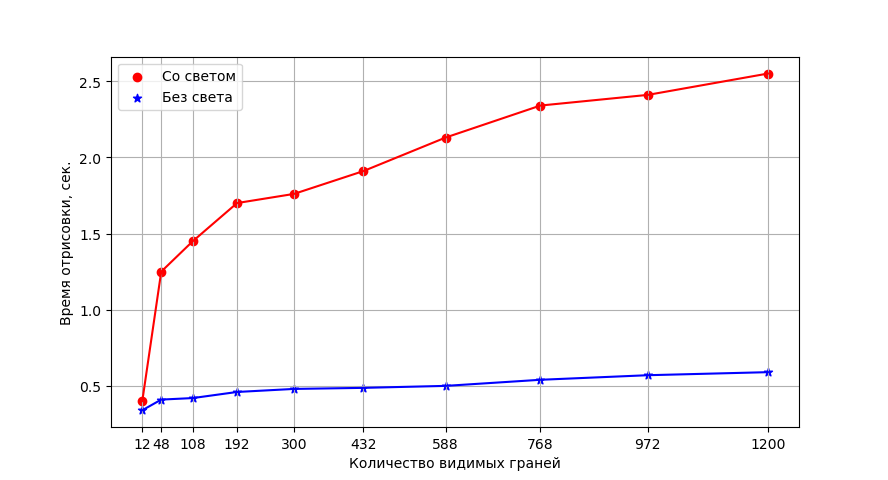
\includegraphics[width=0.7\textwidth]{inc/img/research}
    \caption{Зависимость времени отрисовки кадра от количества граней на сцене}
    \label{fig:inc-img-science}
\end{figure}

%\includeimage
%{research}
%{f}
%{h}
%{0.9\textwidth}
%{Зависимость времени отрисовки кадра от количества граней на сцене}

\clearpage


\section{Вывод}

В данном разделе были приведены технические характеристики устройства,
на котором проводилось измерение времени работы программного обеспечения, а
также результаты замеров времени.

Без учета освещенности алгоритм Z-буфер работает быстрее, чем с учетом освещенности.
Это связано с тем, что для каждого источника света необходимо проинициализировать
и заполнить теневой Z-буфер, а потом для каждого пикселя при растеризации
грани выполнять преобразование координат в координаты в теневом Z-буфере для
определения теней.



\chapter*{ЗАКЛЮЧЕНИЕ}
\addcontentsline{toc}{chapter}{ЗАКЛЮЧЕНИЕ}

В ходе выполнения курсовой работы цель курсовой работы была достигнута:
было разработано программное обеспечение для моделирования сцены улицы из
разработанной библиотеки объектов с возможностью изменять положение камеры
и источника света.

Для достижения цели курсовой работы были решены следующие задачи:
\begin{itemize}
    \item выбраны алгоритмы компьютерной графики для визуализации трехмерной
        сцены;
    \item выбран язык программирования и среда разработки;
    \item разработано программное обеспечение и реализованы выбранные
        алгоритмы визуализации;
    \item проведены замеры временных характеристик
        разработанного программного обеспечения.
\end{itemize}


\makebibliography

\begin{appendices}
	\chapter{}
\end{appendices}


\includepdf[pages=-, fitpaper=true, angle=90]{inc/pdf/presentation.pdf}

\end{document}
